\chapter{Diagramy}

\section{Wprowadzenie}

W poniższym rozdziale przedstawione zostały diagramy sekwencji i klas opisujące tworzoną przez nas aplikację. 

Diagramy sekwencji przedstawiają zależności czasowe pomiędzy obiektami oraz służą do modelowania systemów czasu rzeczywistego i złożonych scenariuszy\footnote{\url{https://pl.wikipedia.org/wiki/Diagram_interakcji}}. Natomiast diagramy klas pokazują określony fragment struktury systemu. Diagramów klas używa się do modelowania statycznych aspektów perspektywy projektowej. Wiąże się z tym silnie modelowanie słownictwa systemu, kooperacji lub schematów. Diagramy klas pozwalają na sformalizowanie specyfikacji danych i metod. Mogą także pełnić rolę graficznego środka pokazującego szczegóły implementacji klas\footnote{\url{https://pl.wikipedia.org/wiki/Diagram_klas}}.
\newpage
\section{Diagram sekwencji}

\begin{figure}[h]
    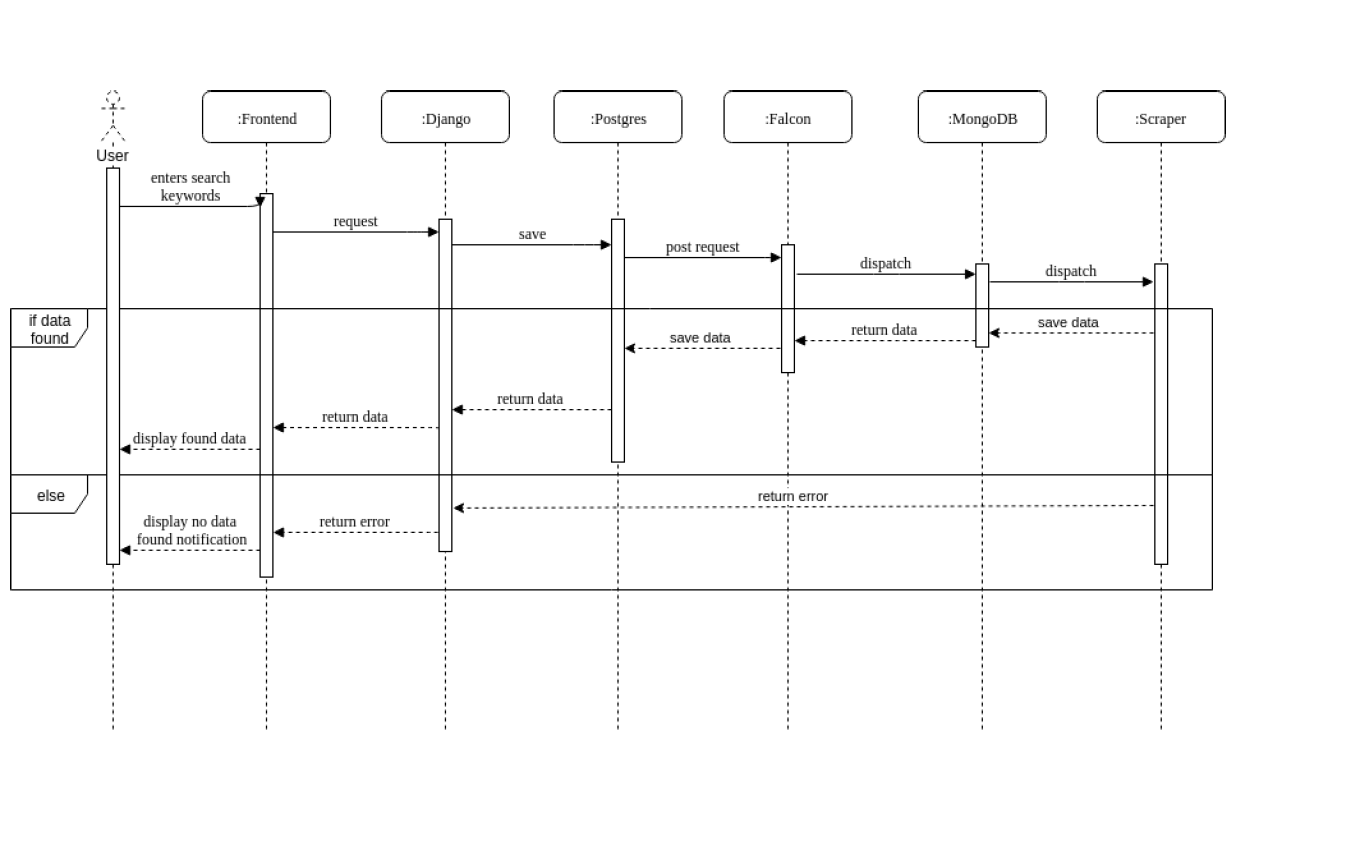
\includegraphics[width=1.10\textwidth]{zdjecia/sekwencja}
    \caption{Diagram sekwencji. Opracowanie własne}
\end{figure}
\newpage

\section{Diagram klas}

\begin{figure}[h]
    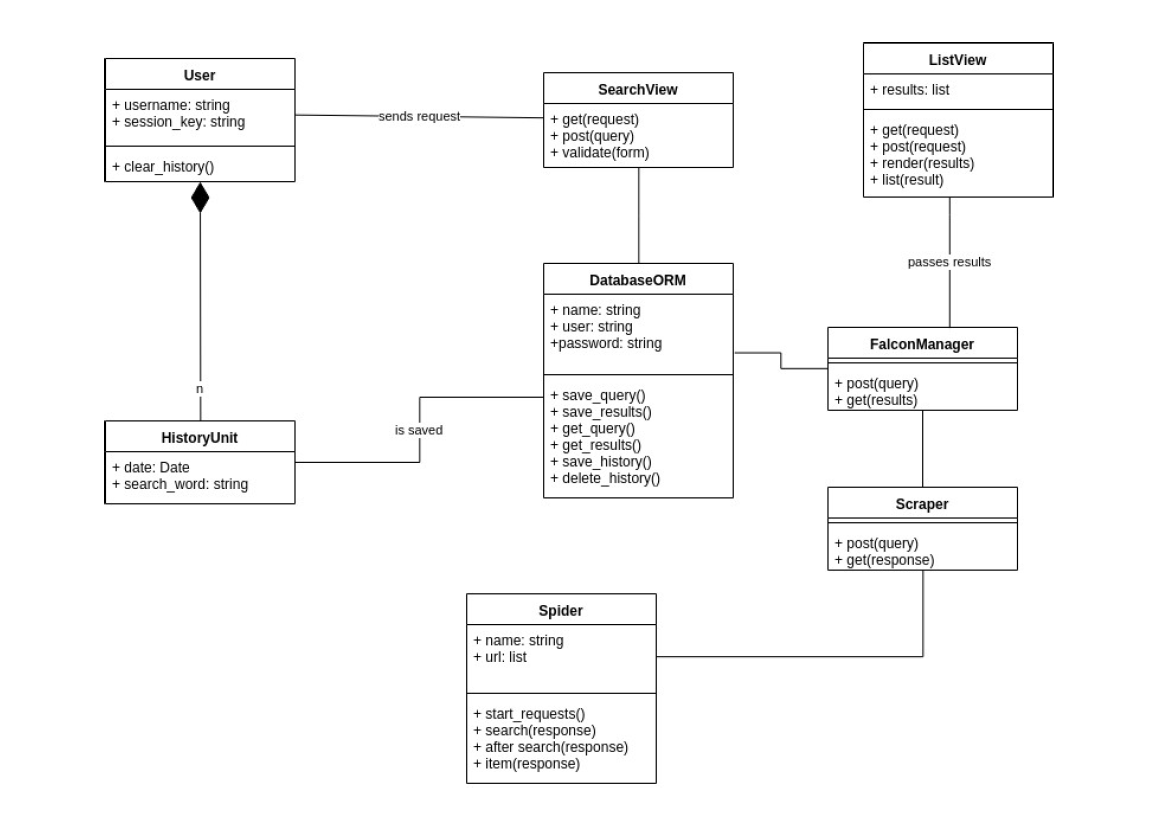
\includegraphics[width=1.10\textwidth]{zdjecia/klas}
    \caption{Diagram klas. Opracowanie własne}
\end{figure}
